\documentclass[12pt,titlepage]{article}
\usepackage[margin=1in]{geometry}
\usepackage{graphicx,amsmath,blindtext}

%% Variables definition
\newcommand{\vSubject}{Basic Programming}
\newcommand{\vSubtitle}{Assignment 6}
\newcommand{\vName}{Dicha Zelianivan Arkana}
\newcommand{\vNIM}{2241720002}
\newcommand{\vClass}{1i}
\newcommand{\vDepartment}{Information Technology}
\newcommand{\vStudyProgram}{D4 Informatics Engineering}

%% [START] Tikz related stuff
\usepackage{tikz}
\usetikzlibrary{svg.path,calc,shapes.geometric,shapes.misc}
\tikzstyle{terminator} = [rectangle, draw, text centered, rounded corners = 1em, minimum height=2.5em]
\tikzstyle{preparation} = [chamfered rectangle, chamfered rectangle sep=0.75em, draw, text centered, minimum height = 2em]
\tikzstyle{process} = [rectangle, draw, text centered, minimum height=2em]
\tikzstyle{decision} = [diamond, aspect=2, draw, text centered, minimum height=2em]
\tikzstyle{data}=[trapezium, draw, text centered, trapezium left angle=60, trapezium right angle=120, minimum height=2em]
\tikzstyle{connector} = [line width=0.25mm,->]
%% [END] Tikz related stuff

%% [START] Fancy header related stuff
\usepackage{fancyhdr}
\pagestyle{fancy}
\setlength{\headheight}{15pt} % compensate fancyhdr style
\fancyhead{}
\fancyfoot{}
\fancyfoot[L]{\thepage}
\fancyfoot[R]{\textit{\vSubject - \vSubtitle}}
\renewcommand{\footrulewidth}{0.4pt}% default is 0pt, overline for footer
%% [END] Fancy header related stuff

%% [START] Custom tabular command related stuff
\usepackage{tabularx}
\newcommand{\details}[2]{
    #1 & #2  \\
}
%% [END] Custom tabular command related stuff

%% [START] Figure related stuff
\newcommand{\image}[3][1]{
    \begin{figure}[h]
        \centering
        \includegraphics[#1]{#2}
        \caption{#3}
        \label{#3}
    \end{figure}
}
%% [END] Figure related stuff

\begin{document}
\begin{titlepage}
    \centering
    \vfill
    {\bfseries\LARGE
        \vSubject\\
        \vskip0.25cm
        \vSubtitle
    }
    \vfill
    
\includegraphics[width=6cm]{images/polinema-logo.png}
    \vfill
    {
        \textbf{Name}\\
        \vName\\
        \vskip0.5cm
        \textbf{NIM}\\
        \vNIM\\
        \vskip0.5cm
        \textbf{Class}\\
        \vClass\\
        \vskip0.5cm
        \textbf{Department}\\
        \vDepartment\\
        \vskip0.5cm
        \textbf{Study Program}\\
        \vStudyProgram
    }
\end{titlepage}

\section*{Assignment 1}
JNX expedition serves domestic and international shipments with the
following details:
\begin{itemize}
    \item {
        For domestic shipments, if the weight of the goods is less than 5 kg then
        there is no charge, if the goods weigh 5-10 kg then a fee of IDR 165,000 is
        charged, and if the weight of the goods is more than 10 kg then a fee of
        IDR 375,000
    }
    \item {
        For international shipments, if the weight of the goods is less than 2 kg,
        there is no charge, if the weight of the goods is more than 2 kg, a fee of
        IDR 500,000 is charged.
    }
\end{itemize}
Create a flowchart to determine the shipping costs that must be paid by customers!

\begin{center}
    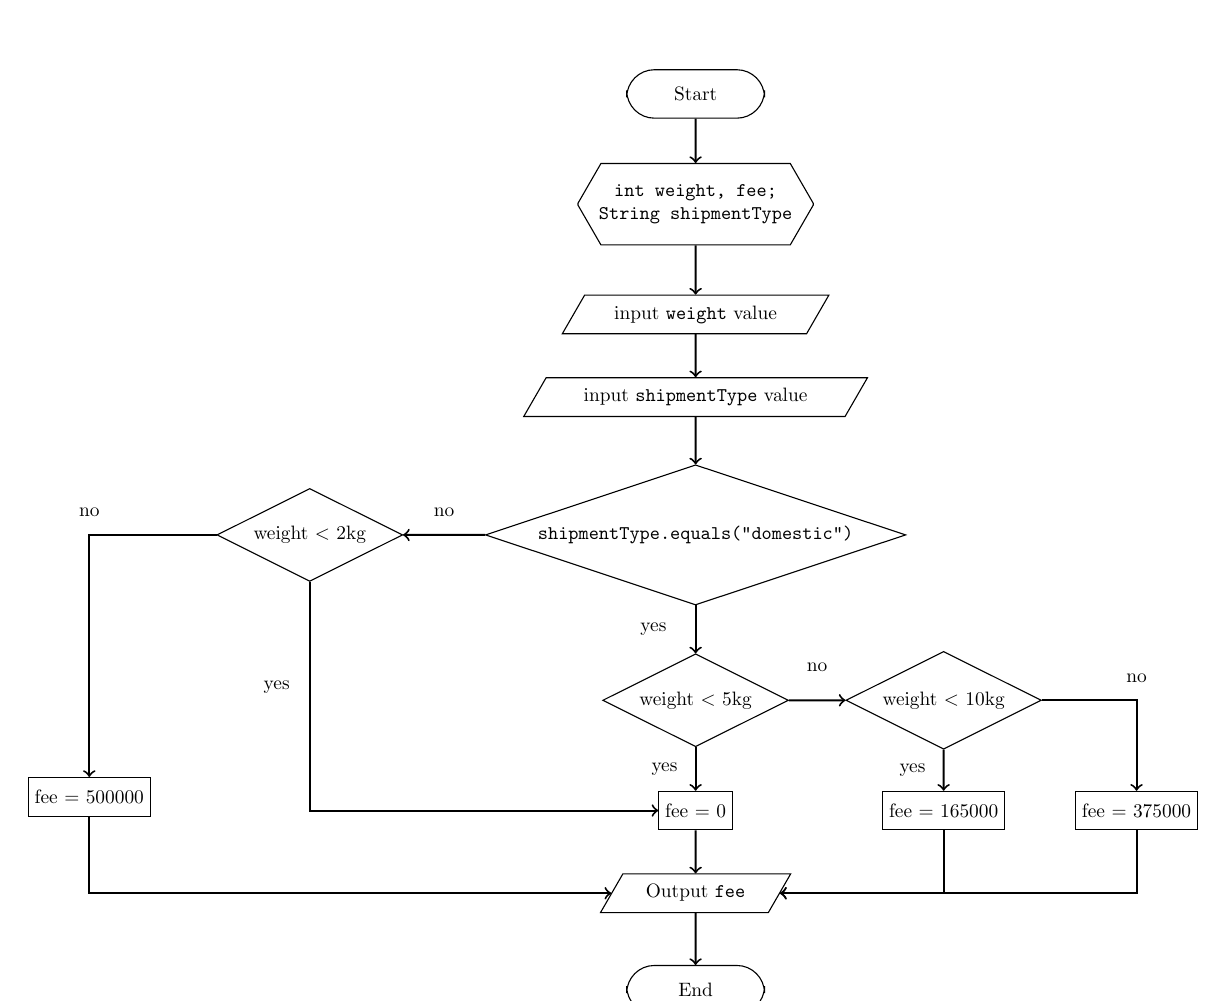
\begin{tikzpicture}[every text node part/.style={align=center}, scale=0.7, every node/.style={scale=0.7}]
        \node (start) [terminator, align=center, minimum width=2.5cm] {Start};
        \node (prep) [preparation, chamfered rectangle angle=30, below of = start, yshift = -1cm] {\texttt{int weight, fee;} \\ \texttt{String shipmentType}};
        \node (input-1) [data, below of = prep, yshift = -1cm] {input \texttt{weight} value};
        \node (input-2) [data, below of = input-1, yshift = -5mm] {input \texttt{shipmentType} value};
        \node (branch-type) [decision, below of = input-2, yshift = -1.5cm, aspect=3] {\texttt{shipmentType.equals("domestic")}};
        \node (branch-domestic-1) [decision, below of = branch-type, yshift = -2cm] {weight $<$ 5kg};
        \node (branch-domestic-2) [decision, right of = branch-domestic-1, xshift = 3.5cm] {weight $<$ 10kg};
        \node (fee-1) [process, below of = branch-domestic-1, yshift=-1cm] {fee = 0};
        \node (fee-2) [process, below of = branch-domestic-2, yshift=-1cm] {fee = 165000};
        \node (fee-3) [process, below of = branch-domestic-2, yshift=-1cm, xshift = 3.5cm] {fee = 375000};
        \node (branch-international) [decision, left of = branch-type, xshift = -6cm] {weight $<$ 2kg};
        \node (fee-int-1) [process, left of = branch-international, xshift = -3cm, yshift = -4.75cm] {fee = 500000};
        \node (output) [data, below of = fee-1, yshift = -5mm] {Output \texttt{fee}};
        \node (end) [terminator, align=center, below of = output, minimum width=2.5cm, yshift = -0.75cm] {End};
        \draw [connector] (start) -- (prep);
        \draw [connector] (prep) -- (input-1);
        \draw [connector] (input-1) -- (input-2);
        \draw [connector] (input-2) -- (branch-type);
        \draw [connector] (branch-type) -- node[left=4mm] {yes} (branch-domestic-1);
        \draw [connector] (branch-domestic-1) -- node[above=4mm] {no} (branch-domestic-2);
        \draw [connector] (branch-domestic-1) -- node[left=2mm] {yes} (fee-1);
        \draw [connector] (branch-domestic-2) -- node[left=2mm] {yes} (fee-2);
        \draw [connector] (branch-domestic-2.east) -| node[above=2mm] {no} (fee-3);
        \draw [connector] (branch-type) -- node[above=2mm] {no} (branch-international);
        \draw [connector] (branch-international) |- node[left=6mm,above=2cm] {yes} (fee-1);
        \draw [connector] (branch-international.west) -| node[above=2mm] {no} (fee-int-1.north);
        \draw [connector] (fee-1) -- (output);
        \draw [connector] (fee-2) |- (output);
        \draw [connector] (fee-3) |- (output);
        \draw [connector] (fee-int-1) |- (output);
        \draw [connector] (output) -- (end);
    \end{tikzpicture}
\end{center}

\pagebreak

\section{Assignment 2}
The ATM system has 3 menus, namely Withdrawal, Transfer, and Change PIN
\begin{itemize}
    \item {
        On the Withdrawal menu, users are asked to select the type of savings
        “Giro” or “Deposito”, then enter the amount of money to be withdrawn
    }
    \item {
        On the Transfer menu, users are asked to select the destination bank code
        consisting of BRI, BNI, Mandiri, Bukopin, and BCA, then enter the
        destination account, and enter the amount of money to be transferred
    }
    \item {
        On the Change PIN menu, the user is asked to enter the old password and
        the new password
    }
\end{itemize}
Make a flowchart for the ATM system!

\begin{center}
    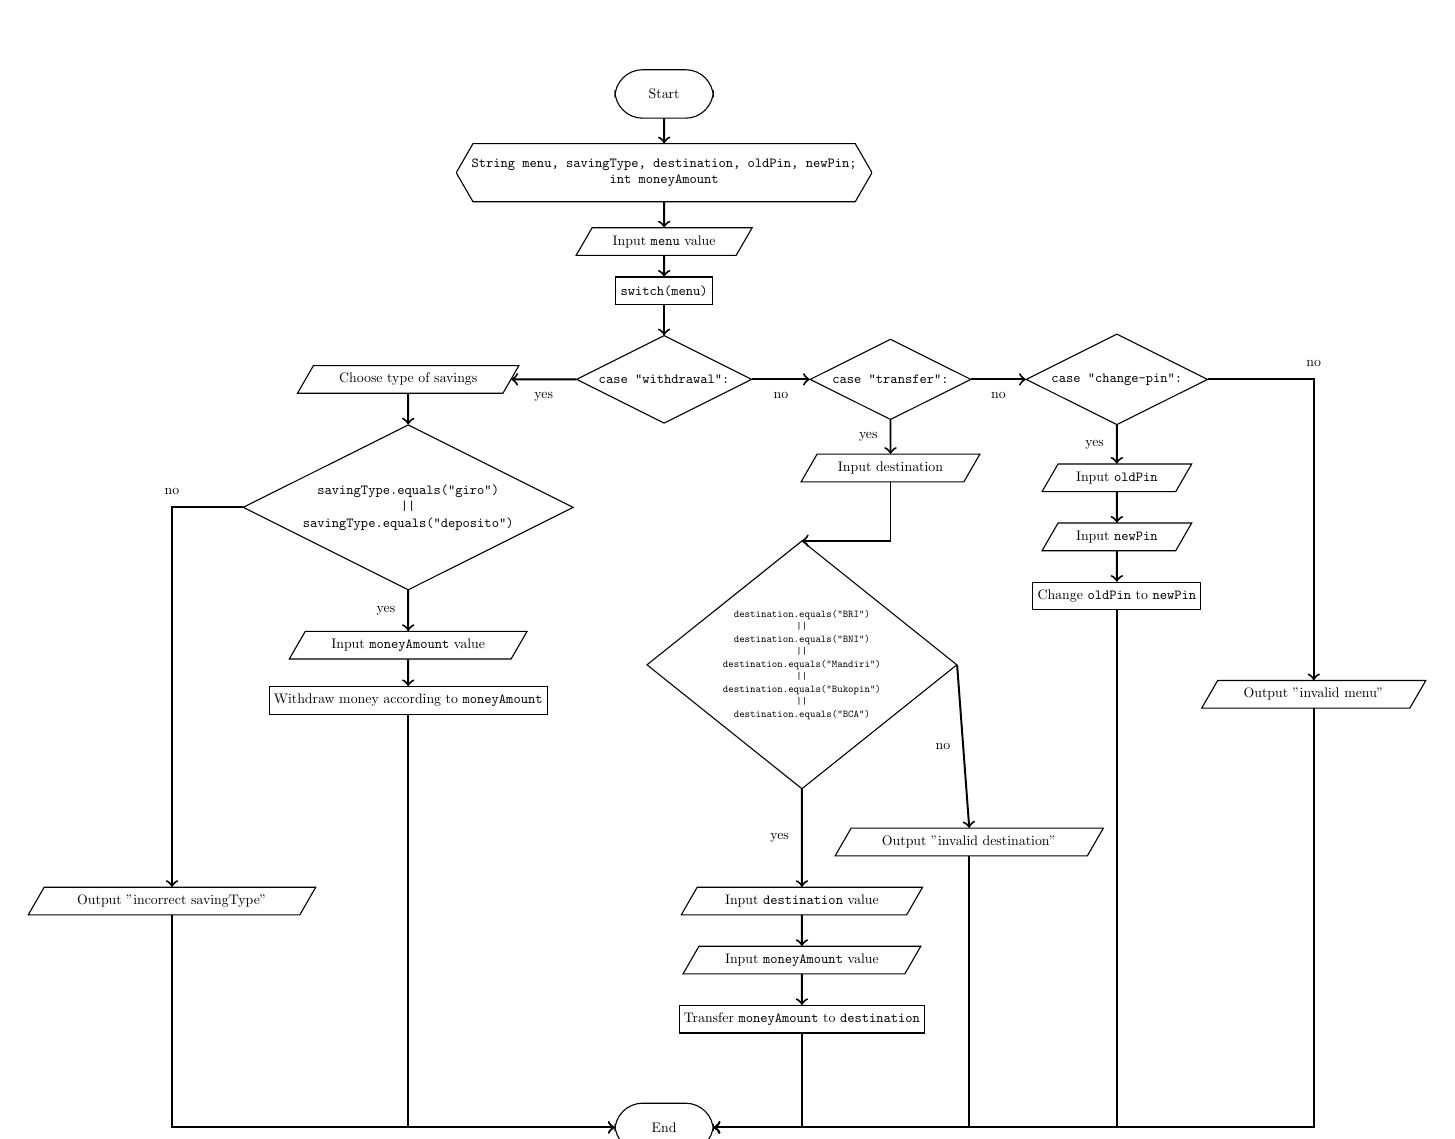
\begin{tikzpicture}[every text node part/.style={align=center}, scale=0.5, every node/.style={scale=0.5}]
        \node (start) [terminator, align=center, minimum width=2.5cm, minimum height=3.5em] {Start};
        \node (prep) [preparation, chamfered rectangle angle=30, below of = start, yshift = -1cm] {\texttt{String menu, savingType, destination, oldPin, newPin;} \\ \texttt{int moneyAmount}};
        \node (input-1) [data, below of = prep, yshift = -7.5mm] {Input \texttt{menu} value};
        \node (switch) [process, below of = input-1, yshift = -2.5mm] {\texttt{switch(menu)}};
        \node (withdrawal) [decision, below of = switch, yshift = -1.25cm] {\texttt{case "withdrawal":}};
        \node (transfer) [decision, right of = withdrawal, xshift = 4.75cm] {\texttt{case "transfer":}};
        \node (change-pin) [decision, right of = transfer, xshift = 4.75cm] {\texttt{case "change-pin":}};
        \node (invalid-menu) [data, right of = change-pin, yshift = -8cm, xshift = 4cm] {Output "invalid menu"}; 
        \node (withdrawal-input) [data, left of = withdrawal, xshift = -5.5cm] {Choose type of savings};
        \node (withdrawal-type) [decision, below of = withdrawal-input, yshift = -2.25cm] {\texttt{savingType.equals("giro")} \\ \texttt{||} \\ \texttt{savingType.equals("deposito")}};
        \node (withdrawal-wrong) [data, left of = withdrawal-type, xshift = -5cm, yshift = -10cm] {Output "incorrect savingType"};
        \node (withdrawal-input-money) [data, below of = withdrawal-type, yshift = -2.5cm] {Input \texttt{moneyAmount} value};
        \node (withdrawal-process) [process, below of = withdrawal-input-money, yshift = -4mm] {Withdraw money according to \texttt{moneyAmount}};
        \node (transfer-input) [data, below of = transfer, yshift = -1.25cm] {Input destination};
        \node (transfer-check-destination) [decision, below of = transfer-input, yshift = -4cm, aspect = 1.25, scale=0.75, xshift = -3cm] {
            \texttt{destination.equals("BRI")} \\
            \texttt{||} \\
            \texttt{destination.equals("BNI")} \\
            \texttt{||} \\
            \texttt{destination.equals("Mandiri")} \\
            \texttt{||} \\
            \texttt{destination.equals("Bukopin")} \\
            \texttt{||} \\
            \texttt{destination.equals("BCA")}
        };
        \node (transfer-invalid-destination) [data, right of = transfer-check-destination, xshift = 3.25cm, yshift = -4.5cm] {Output "invalid destination"};
        \node (transfer-destination-account) [data, below of = transfer-check-destination, yshift = -5cm] {Input \texttt{destination} value};
        \node (transfer-money) [data, below of = transfer-destination-account, yshift = -5mm] {Input \texttt{moneyAmount} value};
        \node (transfer-process) [process, below of = transfer-money, yshift = -5mm] {Transfer \texttt{moneyAmount} to \texttt{destination}};
        \node (change-pin-old) [data, below of = change-pin, yshift = -1.5cm] {Input \texttt{oldPin}};
        \node (change-pin-new) [data, below of = change-pin-old, yshift = -5mm] {Input \texttt{newPin}};
        \node (change-pin-process) [process, below of = change-pin-new, yshift = -5mm] {Change \texttt{oldPin} to \texttt{newPin}};
        \node (end) [terminator, align=center, below of = withdrawal, minimum width = 2.5cm, yshift = -18cm, minimum height=3.5em] {End};
        \draw [connector] (start) -- (prep);
        \draw [connector] (prep) -- (input-1);
        \draw [connector] (input-1) -- (switch);
        \draw [connector] (switch) -- (withdrawal);
        \draw [connector] (withdrawal) -- node[below=2mm] {no} (transfer);
        \draw [connector] (transfer) -- node[below=2mm] {no} (change-pin);
        \draw [connector] (change-pin.east) -| node[above=2mm] {no} (invalid-menu.north);
        \draw [connector] (invalid-menu.south) |- (end.east);
        \draw [connector] (withdrawal.west) -- node[below=2mm] {yes} (withdrawal-input);
        \draw [connector] (withdrawal-input) -- (withdrawal-type);
        \draw [connector] (withdrawal-type.west) -| node[above=2mm] {no} (withdrawal-wrong.north);
        \draw [connector] (withdrawal-wrong) |- (end);
        \draw [connector] (withdrawal-type) -- node[left=2mm] {yes} (withdrawal-input-money);
        \draw [connector] (withdrawal-input-money) -- (withdrawal-process);
        \draw [connector] (withdrawal-process) |- (end);
        \draw [connector] (transfer) -- node[left=2mm] {yes} (transfer-input);
        \draw [connector] (transfer-input) |- (transfer-check-destination.north);
        \draw [connector] (transfer-check-destination) -- node[left=2mm] {yes} (transfer-destination-account);
        \draw [connector] (transfer-check-destination.east) -- node[left=2mm] {no} (transfer-invalid-destination.north);
        \draw [connector] (transfer-invalid-destination.south) |- (end.east);
        \draw [connector] (transfer-destination-account) -- (transfer-money);
        \draw [connector] (transfer-money) -- (transfer-process);
        \draw [connector] (transfer-process) |- (end);
        \draw [connector] (change-pin) -- node[left=2mm] {yes} (change-pin-old);
        \draw [connector] (change-pin-old) -- (change-pin-new);
        \draw [connector] (change-pin-new) -- (change-pin-process);
        \draw [connector] (change-pin-process) |- (end);
    \end{tikzpicture}
\end{center}

\pagebreak

\section{Assignment 3}
Every Saturday, a clothing store gives a discount to its customers according to the
type of clothes and the number of clothes purchased
\begin{itemize}
    \item {
        A 10\% discount is given if the clothes purchased are jackets, then an additional
        2\% discount will be given if more than 2 clothes are purchased
    }
    \item {
        A discount of 7\% is given if the clothes purchased are shirts, then an additional
        2\% discount will be given if the clothes purchased are more than 3, whereas if
        the clothes purchased are less than or equal to 3, an additional 1\% discount will
        be given
    }
    \item {
        Customers will get a 5\% discount for clothes other than jackets and shirts if the
        clothes purchased are more than 3 products
    }
\end{itemize}
Make a flowchart to determine the total amount to be paid if the input is the type
and quantity of clothes (the price of each garment is determined by the system)!

\begin{center}
    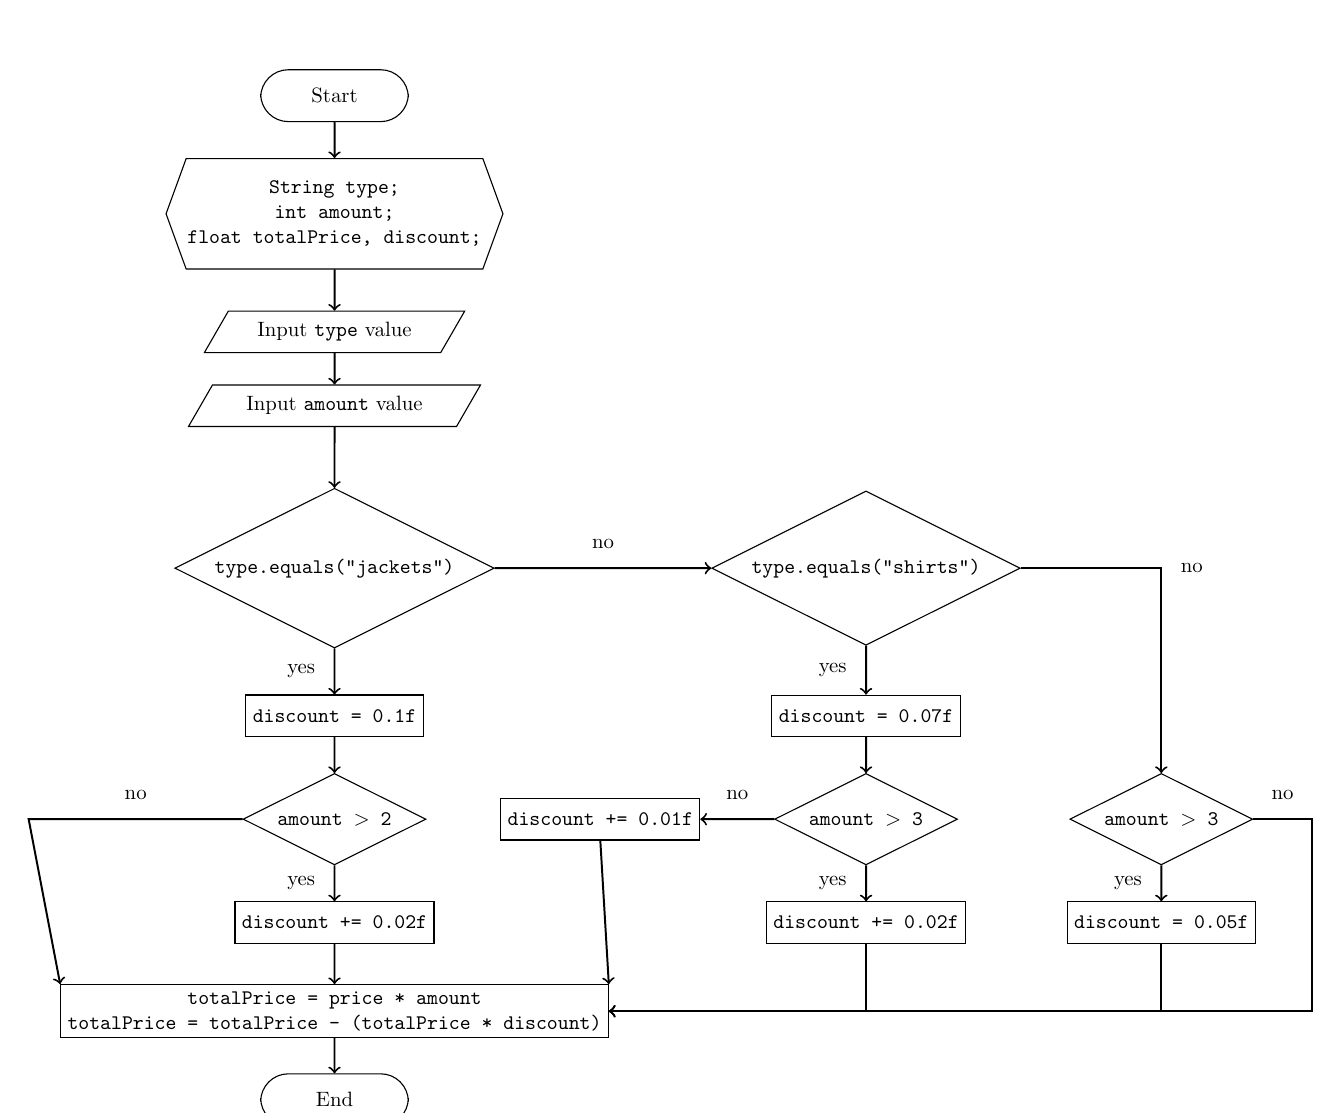
\begin{tikzpicture}[every text node part/.style={align=center}, scale=0.75, every node/.style={scale=0.75}]
        \node (start) [terminator, align=center, minimum width=2.5cm, minimum height=2.5em] {Start};
        \node (prep) [preparation, below of = start, chamfered rectangle angle=20, yshift = -1cm, minimum width = 14em] {
            \texttt{String type;} \\
            \texttt{int amount;} \\
            \texttt{float totalPrice, discount;}
        };
        \node (type-input) [data, below of = prep, yshift = -1cm] {Input \texttt{type} value};
        \node (amount-input) [data, below of = type-input, yshift = -2.5mm] {Input \texttt{amount} value};
        \node (jackets) [decision, below of = amount-input, yshift = -1.75cm] {\texttt{type.equals("jackets")}};
        \node (jackets-discount) [process, below of = jackets, yshift = -1.5cm] {\texttt{discount = 0.1f}};
        \node (jackets-amount) [decision, below of = jackets-discount, yshift = -7.5mm] {\texttt{amount $>$ 2}};
        \node (jackets-discount-gt) [process, below of = jackets-amount, yshift = -7.5mm] {\texttt{discount += 0.02f}};
        \node (shirts) [decision, right of = jackets, xshift = 8cm] {\texttt{type.equals("shirts")}};
        \node (shirts-discount) [process, below of = shirts, yshift = -1.5cm] {\texttt{discount = 0.07f}};
        \node (shirts-amount) [decision, below of = shirts-discount, yshift = -7.5mm] {\texttt{amount $>$ 3}};
        \node (shirts-discount-gt) [process, below of = shirts-amount, yshift = -7.5mm] {\texttt{discount += 0.02f}};
        \node (shirts-discount-lt) [process, left of = shirts-amount, xshift = -3.5cm] {\texttt{discount += 0.01f}};
        \node (other-amount) [decision, right of = shirts, xshift = 4cm, yshift = -4.25cm] {\texttt{amount $>$ 3}};
        \node (other-discount-gt) [process, below of = other-amount, yshift = -7.5mm] {\texttt{discount = 0.05f}};
        \node (calculate) [process, below of = jackets-discount-gt, yshift = -5mm] {
            \texttt{totalPrice = price * amount} \\
            \texttt{totalPrice = totalPrice - (totalPrice * discount)}
        };
        \node (end) [terminator, align=center, below of = calculate, minimum width = 2.5cm, minimum height=2.5em, yshift = -5mm] {End};
        \draw [connector] (start) -- (prep);
        \draw [connector] (prep) -- (type-input);
        \draw [connector] (type-input) -- (amount-input);
        \draw [connector] (amount-input) -- (jackets);
        \draw [connector] (jackets) -- node[left=2mm] {yes} (jackets-discount);
        \draw [connector] (jackets) -- node[above=2mm] {no} (shirts);
        \draw [connector] (shirts) -- node[left=2mm] {yes} (shirts-discount);
        \draw [connector] (shirts.east) -| node[right=2mm] {no} (other-amount.north);
        \draw [connector] (jackets-discount) -- (jackets-amount);
        \draw [connector] (jackets-amount) -- node[left=2mm] {yes} (jackets-discount-gt);
        \draw [connector] (jackets-amount.west) -- node[above=2mm] {no} ($(jackets-amount.west)-(3.625cm,0)$) -- (calculate.north west);
        \draw [connector] (shirts-discount) -- (shirts-amount);
        \draw [connector] (shirts-amount) -- node[left=2mm] {yes} (shirts-discount-gt);
        \draw [connector] (shirts-amount) -- node[above=2mm] {no} (shirts-discount-lt);
        \draw [connector] (other-amount) -- node[left=2mm] {yes} (other-discount-gt);
        \draw [connector] (other-amount.east) -- node[above=2mm] {no} ($(other-amount.east)-(-1cm,0)$) |- (calculate.east);
        \draw [connector] (jackets-discount-gt) -- (calculate);
        \draw [connector] (shirts-discount-gt) |- (calculate);
        \draw [connector] (shirts-discount-lt.south) -- (calculate.north east);
        \draw [connector] (other-discount-gt) |- (calculate);
        \draw [connector] (calculate) -- (end);
    \end{tikzpicture}
\end{center}


\end{document}

